\chapter{Probing the diffusive behaviour in circular accelerators}\label{ch:probing}

%%%%%%%%%%%%%%%%%%%%%%%%%%%%%%%%%%%%%%%%%%%%%%%%%%%%%%%%%%%%%%%%%%%%%%%%%%%%%%%%
\noindent\textsf{The content of this chapter, with the due adaptations, has resulted in the article by C.\ E.\ Montanari, A.\ Bazzani, M.\ Giovannozzi \textit{\citetitle{our_paper9}}, which has been published on Eur. Phys. J. Plus in November 2022~(Ref.~\cite{our_paper9}).}

In this Chapter, the properties of the FP equation, in particular that of the outgoing current at a boundary condition, are studied in detail by means of analytical models and even more by means of numerical simulations. These analyses lead to the definition of an optimal protocol to extract the information about the diffusion coefficient by performing a sequence of well-chosen variations of the position of the boundary condition. An important part of our {analyses focuses} on the determination of the accuracy and robustness of the proposed protocol, {which are key aspects for an experimental determination of the form of the diffusion coefficient}.

The plan of the Chapter is the following. In Section~\ref{sec:some_considerations}, we analyse some important characteristics of the FP process presented in the previous Chapter, with focus on the outgoing current, its behaviour in various conditions, such as in stationary or semi-stationary equilibrium. In Section~\ref{sec:moving_the_absorbing_barrier}, we discuss how the outgoing currents obtained from outward or inward changes of the position of the boundary condition can be described by our model, and how such currents can be split in two processes with distinct timescales. In Section~\ref{sec:numerical_results}, the results presented in the previous sections are used to define a protocol to reconstruct the diffusion coefficient of the FP process. The results of detailed numerical simulations are presented and discussed, quantifying the performance of the proposed method. Finally, in Section~\ref{sec:conclusions} some conclusions are drawn, whereas detail about the numerical integration of the FP process is discussed in Appendix~\ref{app_sec:numerical_integration_with_crank_nicolson} and some analytical computations are presented in the Appendixes~\ref{app_sec:analytic_estimate_of_the_current_loss} and~\ref{app_sec:outgoing_current_for_a_system_with_infinite_source}.

%%%%%%%%%%%%%%%%%%%%%%%%%%%%%%%%%%%%%%%%%%%%%%%%%%%%%%%%%%%%%%%%%%%%%%%%%%%%%%%%

% \section{The diffusion approach to non-linear dynamics}
% \label{sec:the_diffusion_approach}

% %%%%%%%%%%%%%%%%%%%%%%%%%%%%%%%%%%%%%%%%%%%%%%%%%%%%%%%%%%%%%%%%%%%%%%%%%%%%%%%%

% From Hamiltonian systems' theory, we know that orbit diffusion in phase space is related to the presence of extended weakly-chaotic regions~\cite{froeschle1999weak}. Otherwise, the presence of invariant Kolmogorov--Arnol'd--Moser tori ensures long-term stability of the dynamics~\cite{morbidelli1995connection}.

% In circular particle accelerators, the transverse dynamics is affected by a multitude of unavoidable small random perturbations~\cite{ellison1999noise}, as well as slow modulation of magnet currents and transverse tune ripples that could lead to the formation of these weakly-chaotic regions. Therefore, it is reasonable to assume that the particle motion is described by models of the form 
% \begin{equation}
% H(\theta, I, t)=H_{0}(I)+ \xi(t) H_{1}(\theta, I) \, , 
% \label{hstoc}
% \end{equation}
% where $(I, \theta)$ are action-angle variables and $\xi(t)$ is a continuous stationary stochastic noise with zero mean that represents the effect of the chaotic dynamics. In the case of a small stochastic perturbation if the correlation timescale of the noise $\xi(t)$ is much shorter than the evolution timescale of the unperturbed system, it is possible to describe the evolution of the action density function $\rho(I,t)$ by the FP equation (see, e.g.\ Ref.~\cite{bazzani2020diffusion} for the mathematical details and Ref.~\cite{Montanari:2728138} for an application to a stochastic symplectic map)
% \begin{equation}
%     \frac{\partial \rho (I, t)}{\partial t}=\frac{1}{2} \frac{\partial}{\partial I} {D}(I) \frac{\partial}{\partial I}\, \rho(I, t) \, ,
%     %\frac{\partial \rho (I, t)}{\partial t}=\frac{\varepsilon^{2}}{2} \frac{\partial}{\partial I} {D}(I) \frac{\partial}{\partial I}\, \rho(I, t) \, , 
%     \label{eq:fp}
% \end{equation}
% where the diffusion coefficient reads
% \begin{equation}
% D(I)=\sqrt{\left \langle \left (\frac{\partial H_1}{\partial \theta} \right )^2 \right \rangle}
% \label{qsapp}
% \end{equation}    
% and the operator $\langle\,\rangle$ denotes the average value with respect to the angle variables. {Equation~\eqref{eq:fp} is invariant with respect to a rescaling of the time, provided the diffusion coefficient is also rescaled, i.e.\ if $t \to \epsilon t $ and $D \to \epsilon D$, then the FP equation does not change. This arbitrariness is removed by imposing a normalization to the diffusion coefficient, e.g.\ that it has unitary norm.}

% The stochastic perturbation in Eq.~\eqref{hstoc} models the effect
% of a large weakly-chaotic region in phase space and its amplitude should be related to the non-integrability of the dynamics. We assume, therefore, that its amplitude is related to the functional form provided by the optimal estimate of the perturbative series, according to the Nekhoroshev's theorem~\cite{Turchetti:1990aa,Bazzani:1990aa}. Therefore, the diffusion coefficient has the form
% \begin{equation}
%     %D(I)=c \exp \left[-2\left(\frac{I_\ast}{I}\right)^{\frac{1}{2\kappa}}\right]\, , \qquad \int_{0}^{I_{\mathrm{a}}} D(I) \, \mathrm{d}I = 1 \, , 
%     D(I)\propto\exp \left[-2\left(\frac{I_\ast}{I}\right)^{\frac{1}{2\kappa}}\right]\, , 
%     \label{eq:diffusion}
% \end{equation}
% and the two parameters $\kappa, I_\ast$ in Eq.~\eqref{eq:diffusion} have a physical meaning that stems from the Nekhoroshev's theorem: the exponent $\kappa$ is related to the analytic structure of the perturbative series and the dimensionality of the system, and is supposed to be independent from the intensity of the perturbation themselves~\cite{bazzani2020diffusion}; $I_\ast$ is related to the asymptotic character of the perturbative series. 

% {The model based on the assumption that the beam dynamics is governed by a stochastic Hamiltonian, combined with a functional form of the diffusion coefficient derived from the estimate of the time stability from Nekhoroshev theorem, has been applied to the interpretation of intensity measurements in the LHC at top energy~\cite{bazzani2020diffusion}. An excellent agreement between the data collected and the predictions from the FP model, where the approach consists in fitting the values of the model parameters $I_\ast$ and $\kappa$ to the collected data, has been observed. The same functional form of the stability time from Nekhoroshev theorem has been used to derive a scaling law for the time evolution of the dynamic aperture for the case of a system dominated by nonlinear, single-particle-like effects~\cite{PhysRevE.57.3432,Bazzani:2019csk}. This scaling law is also confirmed by the results of numerical simulations. Based on this scaling law, the functional form of the evolution of the beam intensity has been derived~\cite{PhysRevSTAB.15.024001} and proposed as a technique to measure the dynamic aperture of a circular accelerator. Once again, the experimental validation of this approach was fully successful, as indicated by beam measurements performed at the LHC~\cite{PhysRevAccelBeams.22.034002}. All these very encouraging results suggest that Nekhoroshev theorem provides an efficient description of several aspects of beam dynamics.}





%%%%%%%%%%%%%%%%%%%%%%%%%%%%%%%%%%%%%%%%%%%%%%%%%%%%%%%%%%%%%%%%%%%%%%%%%%%%%%%%
\section{Some considerations on Fokker-Planck processes}\label{sec:some_considerations}

We treat our problem by using the 1D action variable $I$, representing the non-linear invariant of the system. We consider the rescaled action variable $I \to I/\sigma^2$, and express the action in units of {the RMS} beam emittance, and this action will therefore be a dimensionless quantity. {A second natural scale of our problem is given by $I_\ast$, as can be derived from the functional form of the diffusion coefficient~\eqref{eq:diffusion}, and, in fact, in several cases, the analyses presented in the rest of this Chapter will be carried out in terms of the dimensionless variable $I/I_\ast$.}

As for the initial condition for the beam distribution, we use the exponential distribution
\begin{equation}
    \rho_0(I) = \exp(-I) \, , 
    \label{eq:initial_distribution}
\end{equation}
obtained by the transformation of the standard Gaussian distribution in physical variables. We also note that for future analysis, it might be interesting to consider beam distributions made of combinations of exponential distributions, as this could be used to simulate the behaviour of a beam with overpopulated tails.

In Ref.~\cite{bazzani2020diffusion}, a value of $\kappa$ around $0.33$ was found as the best fit to the data measured during experimental studies at the LHC, and for this reason this value is used in the numerical simulations presented in this study, {although this choice does not hint at any universality of this value.} Unless specified, we also consider $\epsilon=1$ in all the simulations.

\subsection{Outgoing current}\label{subsec:outgoing_current}

%%%%%%%%%%%%%%%%%%%%%%%%%%%%%%%%%%%%%%%%%%%%%%%%%%%%%%%%%%%%%%%%%%%%%%%%%%%%%%%%

In a generic diffusive process, the outgoing current at the absorbing boundary condition at $I_\mathrm{a}$ is defined as
\begin{equation}
    J_\mathrm{a}(t) = D(I_\mathrm{a})\pdv{\rho(I, t)}{I} \Bigr|_{(I_\mathrm{a}, t)}\,.
    \label{eq:outgoing_current_definition}
\end{equation}
Equation~\eqref{eq:fp} provides a means to obtain an analytical estimate of the current lost at the absorbing barrier (see Appendix~\ref{app_sec:analytic_estimate_of_the_current_loss} for the mathematical details). We consider the change of variable
\begin{equation}
    x(I) = -\int_I^{I_\mathrm{a}} \frac{1}{D^{1/2}(I')}\,\mathrm{d}I' \,, \quad \rho_x(x,t) = \rho(I, t) \sqrt{D(I)} \,, \quad x_\mathrm{a}=x(I_\mathrm{a})=0 \, ,
    \label{eq:change_of_variable}
\end{equation}
and the FP problem in the Smoluchowsky form
\begin{equation}
    \pdv{\rho_x}{t} = \frac{1}{2}\pdv{x} \dv{V(x)}{x} \rho_x+\frac{1}{2}\pdv[2]{\rho_x}{x} \quad \text{where} \quad V(x) = -\ln\left(D^{1/2}(x)\right) \, .
    \label{eq:smol_and_potential}
\end{equation}

{Assuming an initial distribution of the form $\delta(x - x_0)$, where $x_0 \in ] -\infty, 0]$, and approximating the potential $V(x)$ at $x_0$ as $-\nu \, x$, the following expression for the outgoing current at  $x_a = 0$ is obtained}
\begin{equation}
    J_\mathrm{a}(x_0, t) = \frac{|x_0|}{t\sqrt{2\pi t}}\exp\left(-\frac{(x_0+\frac{\nu}{2}t)^2}{2t}\right) \,,
    \label{eq:thecurrent}
\end{equation}
where $\nu$, the linearization of the potential~\eqref{eq:smol_and_potential} at $x_0$ with $D(I)$ given by Eq.~\eqref{eq:diffusion} in the new coordinates, has the following expression
\begin{equation}
    \nu=\frac{1}{2\kappa}\frac{1}{I(x_0)}\left(\frac{I_\ast}{I(x_0)}\right)^{\frac{1}{2\kappa}}\exp\left[-\left(\frac{I_\ast}{I(x_0)}\right)^{\frac{1}{2\kappa}}\right]\,.
    \label{eq:linearised}
\end{equation}

We remark that Eq.~\eqref{eq:thecurrent} can be applied to a generic distribution $\rho_0$ via a convolution
\begin{equation}
    J_\mathrm{a}(t) = \int J_\mathrm{a}(x,t)\rho_x(x)\,\mathrm{d}x\,.
    \label{eq:current_convolution}
\end{equation}
We also note that Eqs.~\eqref{eq:thecurrent} and~\eqref{eq:linearised} provide inevitably an underestimate of the actual current lost~\cite{montanari:ipac2021:tupab233}, as the actual drift term is a positive increasing function for $I\ll I_\ast$. However, we expect an accurate description of the local behaviour close to the absorbing boundary condition, i.e.\ we obtain a good estimate of the current lost for initial distributions that are close enough to the absorbing barrier at $I=I_\mathrm{a}$. 

%%%%%%%%%%%%%%%%%%%%%%%%%%%%%%%%%%%%%%%%%%%%%%%%%%%%%%%%%%%%%%%%%%%%%%%%%%%%%%%%

\subsection{Stationary system with a constant  source}\label{subsec:system_infinite_regime}

%%%%%%%%%%%%%%%%%%%%%%%%%%%%%%%%%%%%%%%%%%%%%%%%%%%%%%%%%%%%%%%%%%%%%%%%%%%%%%%%

Let us consider a diffusive process within the region $[I_0, I_\mathrm{a}]$, with an absorbing boundary condition $\rho(I_\mathrm{a}, t) = 0$, and $\rho(I_0, t) = 1$ as a constant source over time. Regardless of the shape of the initial distribution $\rho_0$, the system will eventually relax to its equilibrium distribution $\rho_\text{eq}(I)$, characterized by a constant outgoing current at $I_\mathrm{a}$. Such a distribution satisfies the following equation
\begin{equation}
    \pdv{I} D(I) \pdv{I} \rho_{\text{eq}}(I) = 0 \,,
\end{equation}
whose solution is given by
\begin{equation}
    \rho_\text{eq}(I) = \alpha \int_I^{I_\mathrm{a}} \frac{1}{D(x)}\,\mathrm{d}x \,, \quad \alpha = \frac{1}{ \displaystyle{\int_{I_0}^{I_\mathrm{a}} \frac{1}{D(x)}\,\mathrm{d}x}} \, .
    \label{eq:equilibrium_stationary_distribution}
\end{equation}

The relaxed system features a constant outgoing current given by
\begin{equation}
    J_\mathrm{a}(t) = D(I_\mathrm{a})\pdv{\rho_\text{eq}}{I}\Bigr|_{(I_\mathrm{a},t)} = \alpha\,,
    \label{eq:equilibrium_stationary_current}
\end{equation} 
which is directly linked to the integral of the diffusion coefficient. For a Nekhoroshev-like diffusion coefficient, we have the analytical expression
\begin{equation}
    \begin{aligned}
        \rho_\text{eq}(I) &= \alpha \int_I^{I_\mathrm{a}} \exp\left[2\left(\frac{I_\ast}{x}\right)^{\frac{1}{2\kappa}}\right] \,\mathrm{d}x \\
        &= 2\alpha\ \kappa x \left[-2\left(\frac{I_\ast}{x}\right)^{\frac{1}{2\kappa}}\right]^{2\kappa} \Gamma\left(-2\kappa, -2\left(\frac{I_\ast}{x}\right)^{\frac{1}{2\kappa}}\right)\Bigg|_I^{I_\mathrm{a}}\,,
    \end{aligned}
\end{equation}
where $\Gamma$ is the upper incomplete gamma function
\begin{equation}
    \Gamma(s,x) = \int_x^{\infty} t^{s-1}\,e^{-t}\,{\rm d}t \,.
\end{equation}

When the system is out of equilibrium, one can obtain an analytical description of the outgoing current by using the formula in Eq.~\eqref{eq:thecurrent}, where, instead of performing a convolution between Eq.~\eqref{eq:thecurrent} and $\rho_0$, we perform a convolution with $\rho_0 - \rho_\text{eq}$. The resulting outgoing current is added to the constant value $\alpha$ (the mathematical details of such procedures are illustrated in Appendix~\ref{app_sec:outgoing_current_for_a_system_with_infinite_source}).

%%%%%%%%%%%%%%%%%%%%%%%%%%%%%%%%%%%%%%%%%%%%%%%%%%%%%%%%%%%%%%%%%%%%%%%%%%%%%%%%

\subsection{Semi-stationary regime for a real system}
\label{subsec:semi_stationary_regime_for_a_real_system}

%%%%%%%%%%%%%%%%%%%%%%%%%%%%%%%%%%%%%%%%%%%%%%%%%%%%%%%%%%%%%%%%%%%%%%%%%%%%%%%%

When working with a Nekhoroshev-like diffusion coefficient, its exponentially small values for $I \ll I_\ast$ generate a stable-core region with extremely low diffusion rates (see Fig.~\ref{fig:1}). This observation can be shown by computing the time of the maximum of the outgoing current for an initial distribution $\delta(I - I_0)$. We consider the time derivative of Eq.~\eqref{eq:thecurrent}
\begin{equation}
\pdv{J_\mathrm{a}(x_0, t)}{t} = \frac{\sqrt{2} x_0 \left[12 t + \left(\nu t - 2 x_0\right) \left(\nu t + 2 x_0\right)\right] }{16 \sqrt{\pi t^7}}\exp\left(-\frac{(x_0+\frac{\nu}{2}t)^2}{2t}\right)\,,
\end{equation}
which is zero for two values of $t$ of opposite sign, and the positive one is
\begin{equation}
    t_{\text{max}}(x_0) = \frac{2 \left(\sqrt{\nu^{2} x_0^{2} + 9} - 3\right)}{\nu^{2}}\,.
    \label{eq:taumax}
\end{equation}
Considering the diffusion coefficient of Eq.~\eqref{eq:diffusion} in the change of variable Eq.~\eqref{eq:change_of_variable}, we have that
\begin{equation}
    x_0(I_0) = {-}\int_{I_0}^{I_\mathrm{a}} \exp\left[\left(\frac{I_\ast}{I}\right)^{\frac{1}{2\kappa}}\right]\,\mathrm{d}I\,.
    \label{eq:peak_current_time}
\end{equation}

We observe that the modulus of the integral of Eq.~\eqref{eq:peak_current_time} increases exponentially for $I_0 \ll I_\ast$. Likewise, the value of $\nu$, given in Eq.~\eqref{eq:linearised}, decreases exponentially in the same range of values of $I_0$, which characterize a strong exponential variation for $t_\text{max}$ as a function of $I_0$. This fact suggests that the contribution to the outgoing current at an absorbing barrier at time $t$ is mainly determined by the initial conditions near $I_0$, with $t_\text{max}(I_0) \approx t$. Hence, given a generic initial distribution $\rho_0(I)$ and an absorbing boundary condition at $I_\mathrm{a}$, after a transient time $t$, the system relaxes to a condition where the current $J_\mathrm{a}(t)$ is mainly determined by $\rho_0(I_0)$, where $I_0$ satisfies $t_\text{max}(I_0) \approx t$. Considering the exponential increase of $t_\text{max}(I)$, we have a core region that is slowly eroded by the diffusive process. Outside this core region, the system behaves as in a semi-stationary regime, characterized by a very slowly varying source at $I_0$.

The evolution of this semi-stationary process can be approximated by modifying the $\alpha$ term in Eq.~\eqref{eq:equilibrium_stationary_distribution} as
\begin{equation}
    \rho_\mathrm{eq}(I, t) = \alpha(t) \int_I^{I_\mathrm{a}} \frac{1}{D(x)}\,\mathrm{d}x\,,
    \label{eq:semi_stationary_distribution}
\end{equation}
where here $\alpha(t)$ depends on the value of the initial distribution $\rho_0(I_0)$, and can be estimated by
\begin{equation}
    \alpha(t) = \frac{\rho_0\left(I_0(t)\right)}{\displaystyle{ \int_{I_0(t)}^{I_\mathrm{a}} \frac{1}{D(x)}\,\mathrm{d}x}}\,,
    \label{eq:alpha_with_time}
\end{equation}
in which $I_0(t)$ is obtained by inverting Eq.~\eqref{eq:peak_current_time} to determine $I_0(x_0)$, and Eq.~\eqref{eq:taumax} to obtain $x_0(t_\mathrm{max})$. By composing the two functions, $I_0(t)$ is determined.

This behaviour can be observed in Fig.~\ref{fig:3}, where a Nekhoroshev-like diffusive process is simulated for a time long enough to reach the semi-stationary regime. Here, we consider the distribution obtained after prolonging the simulation of the system presented in Fig.~\ref{fig:1} with $\kappa=0.33$, and we compare it to $\rho_\mathrm{eq}$ from Eq.~\eqref{eq:equilibrium_stationary_distribution}, using $\alpha$ obtained from Eq.~\eqref{eq:alpha_with_time}. A global offset between the two curves is observed, which clearly highlights the limits of the approximation. 

\begin{figure*}[htp]
    \centering
    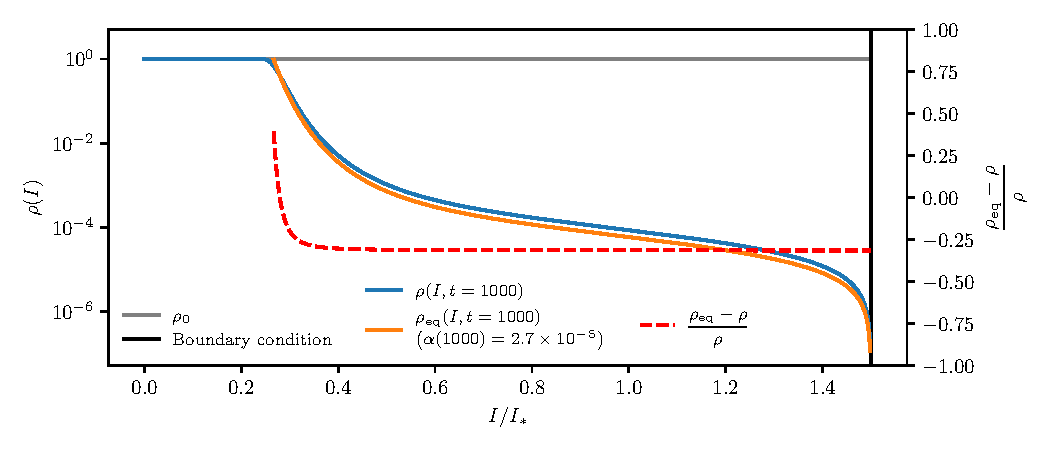
\includegraphics[width=\textwidth]{4_probing_the_diffusive_behavior/figs/final/new_stationary_distribution_s.pdf}
    \caption{Initial uniform distribution for the simulation shown in Fig.~\ref{fig:1} after numerical integration at $t=1000 \, [\text{a. u.}]$, compared to the estimate of $\rho_\mathrm{eq}$ from Eq.~\eqref{eq:equilibrium_stationary_distribution}, with $\alpha(t)$ computed with Eq.~\eqref{eq:alpha_with_time}. (Simulations parameters: $(I_\ast = 1.0\,[\sigma^2],\, \kappa = 0.33)$).}
    \label{fig:3}
\end{figure*}

%%%%%%%%%%%%%%%%%%%%%%%%%%%%%%%%%%%%%%%%%%%%%%%%%%%%%%%%%%%%%%%%%%%%%%%%%%%%%%%%

\section{Reconstruction of the diffusion coefficient of a FP process}
\label{sec:moving_the_absorbing_barrier}

%%%%%%%%%%%%%%%%%%%%%%%%%%%%%%%%%%%%%%%%%%%%%%%%%%%%%%%%%%%%%%%%%%%%%%%%%%%%%%%%

We consider now the problem of modelling the variation of the outgoing current after a change of the position $I_\mathrm{a}$ of the absorbing boundary condition, under the hypothesis that the movement is fast enough to be considered instantaneous, and the movement is performed over a short distance while the system is in the semi-stationary regime described in the previous section. The ultimate goal consists in defining a method for probing the information about the shape of the diffusion coefficient $D(I)$ contained in the outgoing current measured after the instantaneous movement of the boundary condition. This, in view of reconstructing the characteristics of the FP process under analysis, which corresponds to evaluating the values of the two parameters $I_\ast$ and $\kappa$ defining $D(I)$.

We define two types of outgoing current, namely \textsl{global current}, i.e.\ the outgoing current observed from a slow core erosion process while keeping the absorbing boundary condition fixed, and \textsl{recovery current}, i.e.\ the current observed after the absorbing boundary condition is instantaneously moved, and the system relaxes to a new semi-stationary regime.

We start by modelling the shape of the recovery current for a stationary system with a fixed source, both for inward and outward movements of the absorbing boundary. Furthermore, we recall that this mimics what is done experimentally when attempting to measure the diffusion equation by performing scans of the position of some collimators jaws~{\cite{MESS1994279,flilleriii:pac03-rpag004,stancari2011diffusion,stancari:ipac11-tupz033,Stancari:1637929,PhysRevSTAB.16.021003,PhysRevAccelBeams.23.044802}}. Afterwards, we try to adapt the models to a system in semi-stationary regime, characterized by a source evolving with time.

%%%%%%%%%%%%%%%%%%%%%%%%%%%%%%%%%%%%%%%%%%%%%%%%%%%%%%%%%%%%%%%%%%%%%%%%%%%%%%%%

\subsection{Moving the absorbing boundary condition inwards}

%%%%%%%%%%%%%%%%%%%%%%%%%%%%%%%%%%%%%%%%%%%%%%%%%%%%%%%%%%%%%%%%%%%%%%%%%%%%%%%%

Let us consider a system in equilibrium with a constant  source $\rho(I_0, t)=1$, and an absorbing boundary condition $\rho(I_\mathrm{a}, t)=0$, and assume that the boundary condition is instantaneously moved inwards to $\rho(I'_\mathrm{a}, t)=0$, with $I_0 < I'_\mathrm{a} < I_\mathrm{a}$. After this change, the equilibrium distribution varies and the new equilibrium distribution is given by
\begin{equation}
    \rho'_\text{eq}(I) = \beta \int_I^{I'_\mathrm{a}} \frac{1}{D(x)}\,\mathrm{d}x\,,
\end{equation}
where $\beta$ is a constant such  that $\rho'_\text{eq}(I_0)=1$, and when compared with the constant $\alpha$ from Eq.~\eqref{eq:equilibrium_stationary_distribution}, we have that $\alpha < \beta$. The graphs of $\rho_\mathrm{eq}$ and $\rho'_\mathrm{eq}$ are shown in Fig.~\ref{fig:4} (top).

To apply the analytical formulae presented in the previous section, we need to compute the difference distribution $\rho^\ast(I)$. Assuming that the original system starts from the equilibrium distribution in Eq.~\eqref{eq:equilibrium_stationary_distribution}, we obtain 
\begin{align}
    \rho^\ast(I) = \rho_\text{eq}(I) - \rho'_\text{eq}(I) 
    &= \alpha \int_I^{I_\mathrm{a}} \frac{1}{D(x)}\,\mathrm{d}x - \beta \int_I^{I'_\mathrm{a}} \frac{1}{D(x)}\,\mathrm{d}x \notag \\
    &= \alpha \left( 
          \int_{I}^{I'_\mathrm{a}} \frac{1}{D(x)}\,\mathrm{d}x 
        + \int_{I'_\mathrm{a}}^{I_\mathrm{a}} \frac{1}{D(x)}\,\mathrm{d}x \right) - \beta \int_I^{I'_\mathrm{a}} \frac{1}{D(x)}\,\mathrm{d}x \notag \\
    &=  \alpha \int_{I'_\mathrm{a}}^{I_\mathrm{a}} \frac{1}{D(x)}\,\mathrm{d}x \, - (\beta - \alpha) \int_{I}^{I'_\mathrm{a}} \frac{1}{D(x)}\,\mathrm{d}x \notag \\
    &=  \rho^\ast_\text{app} - (\beta - \alpha) \int_{I}^{I'_\mathrm{a}} \frac{1}{D(x)}\,\mathrm{d}x \, .
    \label{eq:inward_difference}
\end{align}

The shape of $\rho^\ast(I)$ is shown in Fig.~\ref{fig:4} (bottom). This function, restricted to the interval $I \in [I_0, I'_\mathrm{a}]$, is monotonously increasing, with the maximum in $I'_\mathrm{a}$. Given the  Nekhoroshev-like form of the diffusion coefficient, the decrease to zero when $I \to I_0$ is exponentially fast, while in the region close to $I'_\mathrm{a}$, the function remains almost constant to the value  $\rho^\ast_\text{app}$ that can be used as the lowest-order approximation of $\rho^\ast(I)$.

\begin{figure*}[htp]
    \centering
    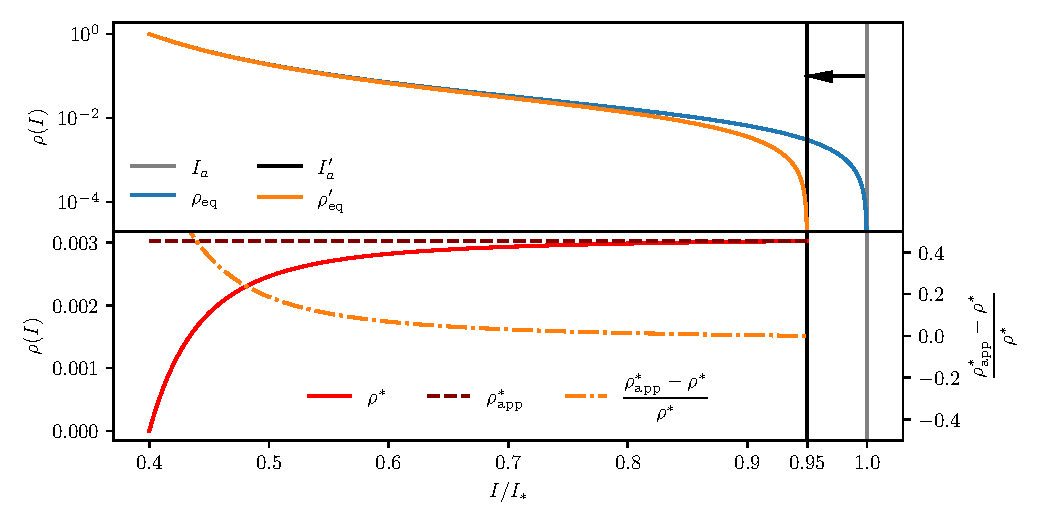
\includegraphics[width=\textwidth]{4_probing_the_diffusive_behavior/figs/final/difference_backwards_s.pdf}
    \caption{Top: Equilibrium distribution for $I_\mathrm{a}/I_\ast = 1.0$ compared with the  equilibrium distribution for $I'_\mathrm{a}/I_\ast = 0.95$. Bottom: Difference between the two equilibrium distributions. (Simulations parameters: $I_\ast = 1.0\,[\sigma^2],\, \kappa = 0.33,\, I_0/I_\ast = 0.4$).}
    \label{fig:4}
\end{figure*}

In Fig.~\ref{fig:5}, we compare the simulated current with its analytical estimate, obtained by computing the convolution with the distribution $\rho^\ast(I)$ of Eq.~\eqref{eq:inward_difference}, which are in very good agreement {(i.e.\ with a difference not greater than $10\%$)}. In the same figure, the analytical approximation based on the convolution with $\rho^\ast_\text{app}$ is shown, and even in this case the agreement is very good {(i.e.\ with a difference not greater than $10\%$)}.

\begin{figure*}[htp]
    \centering
    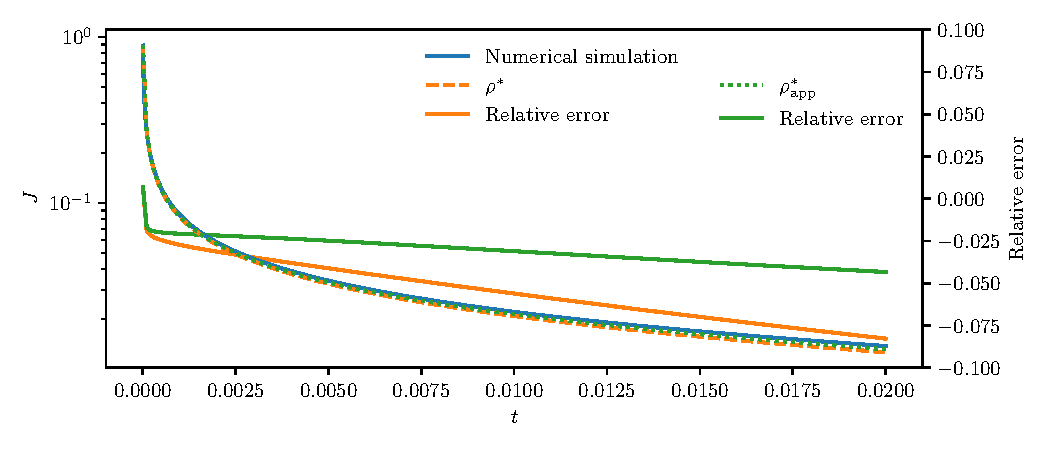
\includegraphics[width=\textwidth]{4_probing_the_diffusive_behavior/figs/final/current_backwards.pdf}
    \caption{Comparison between the current generated by the inward displacement of the absorbing boundary condition shown in Fig.~\ref{fig:4}, its analytical estimate based on $\rho^\ast(I)$, and the analytical estimate based on $\rho^\ast_\text{app}$.}
    \label{fig:5}
\end{figure*}

%%%%%%%%%%%%%%%%%%%%%%%%%%%%%%%%%%%%%%%%%%%%%%%%%%%%%%%%%%%%%%%%%%%%%%%%%%%%%%%%

\subsection{Moving the absorbing boundary condition outwards}

%%%%%%%%%%%%%%%%%%%%%%%%%%%%%%%%%%%%%%%%%%%%%%%%%%%%%%%%%%%%%%%%%%%%%%%%%%%%%%%%

Let us now consider a system in equilibrium with a constant source $\rho(I_0, t)=1$, and an absorbing boundary condition $\rho(I_\mathrm{a}, t)=0$, and assume that this boundary condition is instantaneously moved outwards to $\rho(I''_\mathrm{a}, t)=0$, with $I_0 < I_\mathrm{a} < I''_\mathrm{a}$. The new equilibrium distribution is given by
\begin{equation}
    \rho''_\text{eq}(I) = \gamma \int_I^{I''_\mathrm{a}} \frac{1}{D(x)}\,\mathrm{d}x\,,
\end{equation}
where $\gamma$ is a constant such that $\rho''_\text{eq}(I_0)=1$, and when compared with the constant $\alpha$ from Eq.~\eqref{eq:equilibrium_stationary_distribution}, we have that $\gamma < \alpha$. The graphs of $\rho_\text{eq}(I)$ and $\rho''_\text{eq}(I)$ are shown in Fig.~\ref{fig:6} (top). 

To define properly the difference distribution in the new interval $[I_0, I''_\mathrm{a}]$, we need to extend the definition of the equilibrium distribution $\rho_\text{eq}(I)$, namely
\begin{equation}
    \rho_\text{eq}(I) = 
    \left\{\begin{array}{lr}
        \alpha \displaystyle{\int_I^{I_\mathrm{a}} \frac{1}{D(x)}\,\mathrm{d}x} \qquad & \text{if } \, I \leq I_\mathrm{a} \\
        \\
        0 \qquad & \text{if } \, I > I_\mathrm{a}\,,
    \end{array}\right.\,,
\end{equation}
which leads to the following expression for the difference distribution  
\begin{equation}
    \rho^\ast(I) = 
    \left\{\begin{array}{lr}
        - \gamma \displaystyle{\int_{I_\mathrm{a}}^{I''_\mathrm{a}} \frac{1}{D(x)}\,\mathrm{d}x + (\alpha - \gamma) \int_{I}^{I_\mathrm{a}} \frac{1}{D(x)}\,\mathrm{d}x}\ \quad &\text{if} \, I \leq I_\mathrm{a}\\
        \\
        - \gamma \displaystyle{\int_{I}^{I''_\mathrm{a}} \frac{1}{D(x)}\,\mathrm{d}x} \quad &\text{if} \, I > I_\mathrm{a}\,,
    \end{array}\right. 
    \label{eq:outward_difference}
\end{equation}
which is a negative distribution, with a minimum at $I_\mathrm{a}$ and with $\rho^\ast(I_0) = \rho^\ast(I''_\mathrm{a}) = 0$.

A plot of $\rho^\ast(I)$ is shown in Fig.~\ref{fig:6} (bottom), and we remark that this distribution leads to a negative outgoing current that needs to be combined with the stationary current from the equilibrium process for obtaining the actual outgoing current.

While in the interval $[I_0, I_\mathrm{a}]$ a constant approximated distribution function can be a reasonable assumption, in the interval $[I_\mathrm{a}, I''_\mathrm{a}]$ a different approximation is needed. Under the assumption that the outward step $I''_\mathrm{a} - I_\mathrm{a}$ is small, a linear approximation from $\rho^\ast(I_\mathrm{a})$ to $\rho^\ast(I''_\mathrm{a})$ can be considered, namely
\begin{equation}
    \rho^\ast_\text{app}(I) = 
    \left\{\begin{array}{lr}
        - \gamma \displaystyle{\int_{I_\mathrm{a}}^{I''_\mathrm{a}} \frac{1}{D(x)}\,\mathrm{d}x} \quad &\text{  if } \, I \leq I_\mathrm{a}\\
        \\
        - \gamma \displaystyle{\left(\frac{I''_\mathrm{a} - I}{I''_\mathrm{a} - I_\mathrm{a}} \right)} \displaystyle{\int_{I_\mathrm{a}}^{I''_\mathrm{a}} \frac{1}{D(x)}\,\mathrm{d}x} \quad &\text{  if } \, I > I_\mathrm{a} \,.
    \end{array}\right. 
    \label{eq:outward_difference_approx}
\end{equation} 

\begin{figure*}[htp]
    \centering
    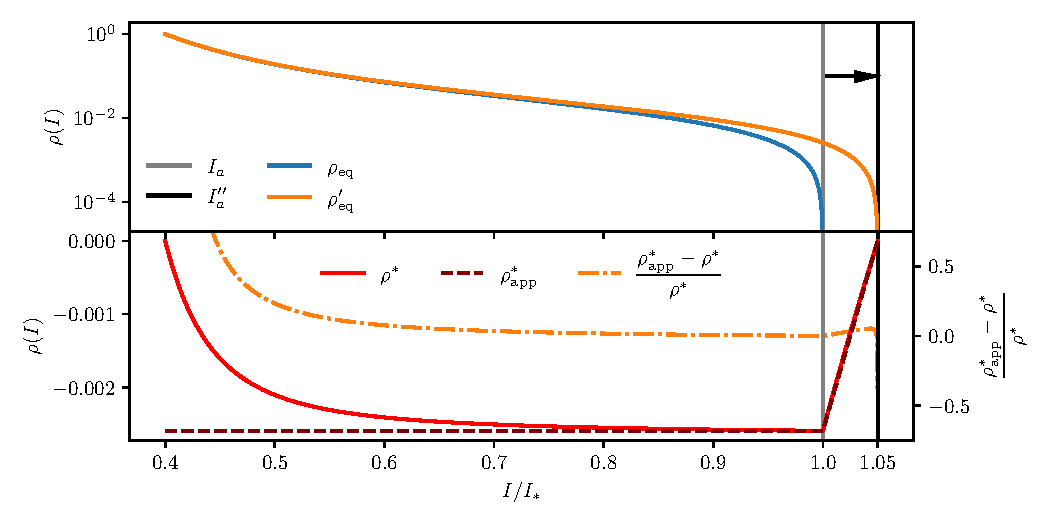
\includegraphics[width=\textwidth]{4_probing_the_diffusive_behavior/figs/final/difference_outwards_s.pdf}
    \caption{Top: Equilibrium distribution for $I_\mathrm{a}/I_\ast = 1.0$ compared with the equilibrium distribution for $I''_\mathrm{a}/I_\ast = 1.05$. Bottom: Difference between the two distributions. (Simulations parameters: $I_\ast = 1.0\,[\sigma^2],\, \kappa = 0.33,\, I_0/I_\ast = 0.4$).}
    \label{fig:6}
\end{figure*}

In Fig.~\ref{fig:7}, we compare the simulated current with its analytical estimate, obtained by computing the convolution with the distribution $\rho^\ast(I)$ of Eq.~\eqref{eq:outward_difference}, which are in good agreement {(i.e.\ with a difference not greater than $10-15\%$)}. In the same figure, the analytical approximation based on the convolution with $\rho^\ast_\text{app}$ is shown, and even in this case the agreement is excellent {(i.e.\ with a difference not greater than $5\%$)}.

\begin{figure*}[htp]
    \centering
    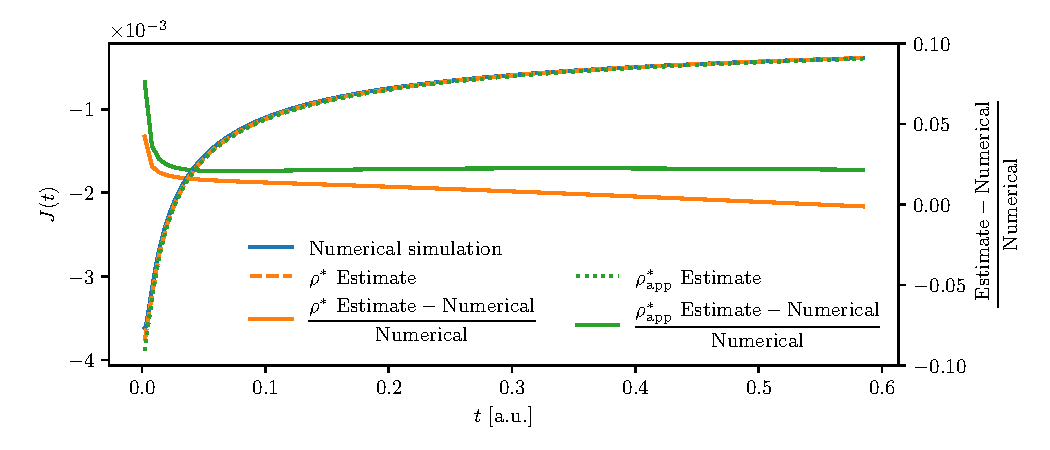
\includegraphics[width=\textwidth]{4_probing_the_diffusive_behavior/figs/final/current_outwards.pdf}
    \caption{Comparison between the current generated by the outward displacement of the absorbing boundary condition shown in Fig.~\ref{fig:6}, its analytical estimate based on $\rho^\ast(I)$, and the analytical estimate based on the approximation $\rho^\ast_\text{app}$.}
    \label{fig:7}
\end{figure*}

%%%%%%%%%%%%%%%%%%%%%%%%%%%%%%%%%%%%%%%%%%%%%%%%%%%%%%%%%%%%%%%%%%%%%%%%%%%%%%%%

\subsection{Moving the absorbing boundary condition in a semi-stationary system}
\label{subsec:Moving_the_boundary_in_a_semi_stationary_system}

%%%%%%%%%%%%%%%%%%%%%%%%%%%%%%%%%%%%%%%%%%%%%%%%%%%%%%%%%%%%%%%%%%%%%%%%%%%%%%%%

In Section~\ref{subsec:semi_stationary_regime_for_a_real_system} we have seen how it is possible to describe a diffusive process, after a transient time, as a semi-stationary process in which a stable core is being slowly eroded over an exponentially-long time, with an approximated timescale given by Eq.~\eqref{eq:peak_current_time}. If the position of the absorbing boundary condition is changed when the system is in this semi-stationary state, and the new position is close to the original one, so that it is characterized by a timescale of the same order of magnitude, the stationary part of the system, i.e.\ the relaxed part outside the stable-core, will relax to a new configuration in a time that is short compared to the timescale of the stable-core erosion.

Being the timescale of the recovery-current process orders of magnitude shorter than the evolution of the global current, the variation of the shape of the core is so slow that it can be neglected. Hence, one can treat this situation as a source at a fixed position with a slow-varying intensity $\alpha(t)$. 

%%%%%%%%%%%%%%%%%%%%%%%%%%%%%%%%%%%%%%%%%%%%%%%%%%%%%%%%%%%%%%%%%%%%%%%%%%%%%%%%

\subsubsection{Normalizing a recovery current}

%%%%%%%%%%%%%%%%%%%%%%%%%%%%%%%%%%%%%%%%%%%%%%%%%%%%%%%%%%%%%%%%%%%%%%%%%%%%%%%%

Thanks to the previous assumptions, one can define a normalization procedure to be applied to the recovery current to make it independent of the characteristics of the global current. We are interested in reducing the problem to the ideal case of a constant source at $I_0$ and a constant unitary outgoing current at the absorbing boundary condition $I_\mathrm{a}$, instead of a system with a slow-varying global current $\alpha(t)$. This approach is tested by simulating the same Nekhoroshev-like FP system twice: firstly, by keeping the absorbing boundary fixed; secondly, by executing some instantaneous changes of the absorbing boundary position. With this approach, we gather information on the value of the semi-stationary current $\alpha(t)$, thus enabling the transformation of the process with a moving boundary to a system with a fixed source.

We define the normalized recovery current as the current obtained in the measurement with the moving absorbing barrier divided by the current $\alpha(t)$, obtained in the measurement with fixed boundary. The normalized recovery current has a unitary value when the absorbing boundary condition is not changed, and has normalized maximum and minimum, respectively, for the inward and outward movements of the absorbing boundary condition. The behaviour of the normalized recovery current can be related to the ideal stationary systems described above, for which analytical approximations are known.

In Fig.~\ref{fig:fixed-vs-moved-boundary}, an example of such a procedure is displayed (centre) together with the evolution of the outgoing current (top) and the corresponding variation of the position of the boundary condition (bottom). It is worth mentioning that for every change of $I_\mathrm{a}$ the value of $\alpha(t)$ changes according to Eq.~\eqref{eq:alpha_with_time}, although for small variations of the absorbing boundary condition, a Taylor expansion can be applied.

\begin{figure*}[htp]
    \centering
    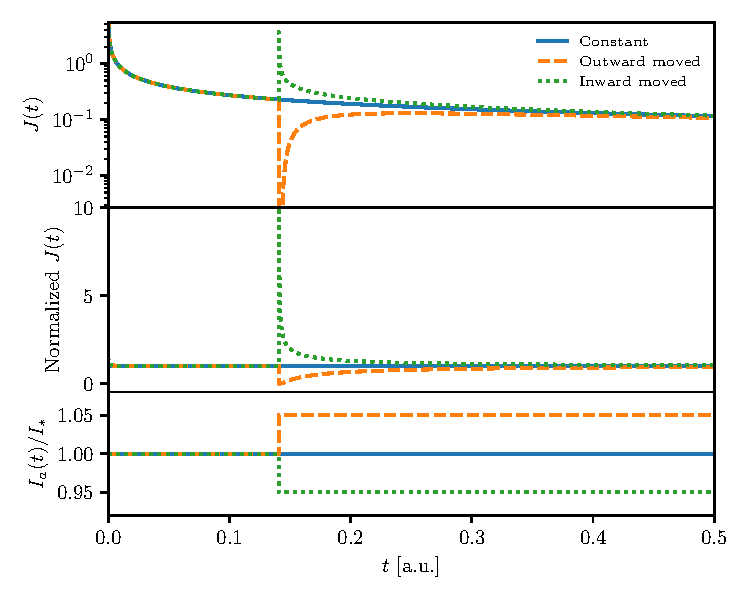
\includegraphics[width=\textwidth]{4_probing_the_diffusive_behavior/figs/final/global_vs_moving_current.pdf}
    \caption{Top: Evolution of the outgoing current for three diffusive processes with different boundary conditions. Middle: Evolution of the normalized outgoing current. Bottom: Changes to the absorbing boundary condition in the three scenarios. (Simulations parameters: $I_\ast = 1.0\,[\sigma^2], \, \kappa = 0.33$).}
    \label{fig:fixed-vs-moved-boundary}
\end{figure*}

%%%%%%%%%%%%%%%%%%%%%%%%%%%%%%%%%%%%%%%%%%%%%%%%%%%%%%%%%%%%%%%%%%%%%%%%%%%%%%%%

\subsubsection{Normalizing a recovery current without knowledge of the global current}

%%%%%%%%%%%%%%%%%%%%%%%%%%%%%%%%%%%%%%%%%%%%%%%%%%%%%%%%%%%%%%%%%%%%%%%%%%%%%%%%

Whenever it is not possible to repeat two complete measurements on the same process, i.e.\ one with and one without changes of the boundary condition position, the normalization procedure defined previously needs to be adapted.

Ideally, the best strategy consists in waiting long enough after each change of the position of the absorbing boundary to reach an equilibrium and to accomplish the recovery process so that the outgoing current measured before the change of boundary position and after the long wait is a pure global current. This would approximately correspond to a complete relaxation of the difference distribution resulting from the boundary movement. Hence, in this way, the outgoing current can be used for reconstructing the shape of the global current and for the normalization procedure.

However, some extra hurdles should be considered: since we do not have a prior knowledge of the value of $D(I)$, we do not know the timescales of the recovery currents or those of the core-eroding process. Moreover, even though a good fraction of the recover process is achieved very quickly, a full recover, corresponding to a full relaxation of the difference distribution $\rho^\ast$, might take an exponentially-long amount of time, possibly beyond computing capabilities. Hence, it might not be possible to perform such a long measurement in a particle accelerator. Therefore, it is necessary to define a protocol that enables quantitative criteria to establish whether or not an assumed recovery time is long enough to ensure a meaningful reconstruction of the behaviour of the FP process, possibly including an estimate of the uncertainty in the reconstruction of the global current.

A possible solution, compatible with these constraints, consists in the combination of three movements of the boundary condition, where, for each value of the action to be probed, an outward-inward-outward sequence of movements is performed. These three steps must be performed with a fixed movement size $\Delta I$ and with a fixed relaxation time $\Delta t$ between a boundary condition movement and the next one. The optimal values for $\Delta I$ and $\Delta t$ are discussed in the next section. A visualization of this protocol is provided in Fig.~\ref{fig:9} (bottom), where the three-step boundary condition change is highlighted and repeated three times, and the corresponding evolution of the outgoing current is given (top), as computed from numerical simulations. As a comparison, the situation corresponding to the constant position of the boundary condition is also shown.

We remark that variants of the proposed three-step movement are indeed possible, and that this proposal is also motivated by the wish not to introduce unnecessary complications. It is also important to stress that the assumption of performing small and equal movements of the absorbing barrier position for the three steps implies that also $\Delta t$ should be the same for the steps, as the relaxation time should be approximately the same for all steps. 

This three-step sequence of absorbing-barrier changes is performed at different values of the global current, and this basic sequence can be repeated by performing it at different action values. The resulting sequence of alternating recovery currents provides an approximation of the evolution of the global current with a sequence of upper- and lower-bound values at different times, which can be interpolated and used for the construction of a global current estimate. These bounds provide a degree of uncertainty directly linked to the chosen value $\Delta t$, as the longer $\Delta t$ is, the lower the degree of uncertainty in the reconstruction of the global current is. A more detailed discussion on a possible quantitative definition of the optimal choice of the relaxation timescale $\Delta t$, together with the effects of using shorter relaxation times, is discussed in the next section.

To reconstruct the global current, an upper- and lower-bound estimate are derived by considering the last values of the inward and outward recovery currents, respectively. Two extra points are added to the upper- and lower-bound estimate, with the goal of covering the maximum time span for reconstructing the global current: the last measured global current value before the first boundary movement is added to both estimates; the last value of the last recovery current measured, which, being an outward recovery current, was already part of the lower-bound estimate, is added also to the upper-bound estimate. This explains why in Fig.~\ref{fig:protocol} (centre) the estimates coincide at the beginning and end of the interpolation interval. The two sets of upper-bound and lower-bound points are each interpolated with a univariate cubic spline and the average function of these two interpolating functions is taken as the estimate of the global current. 

We remark that the univariate cubic spline is taken with a number of knots so that the second derivative does not change in sign. This ensures that the resulting global current estimate fulfils the expected features of the actual global current. In particular, it avoids local oscillations that might be generated by a simple interpolation of the upper-bound and lower-bound points. The result of such an approach is shown in Fig.~\ref{fig:protocol} where a fraction of the data presented in Fig.~\ref{fig:9} is used for reconstructing the global current, and an excellent overall agreement  {(i.e.\ with a difference not greater than $5\%$)} with the actual global current is clearly visible.
%
\begin{figure*}[htp]
    \centering
    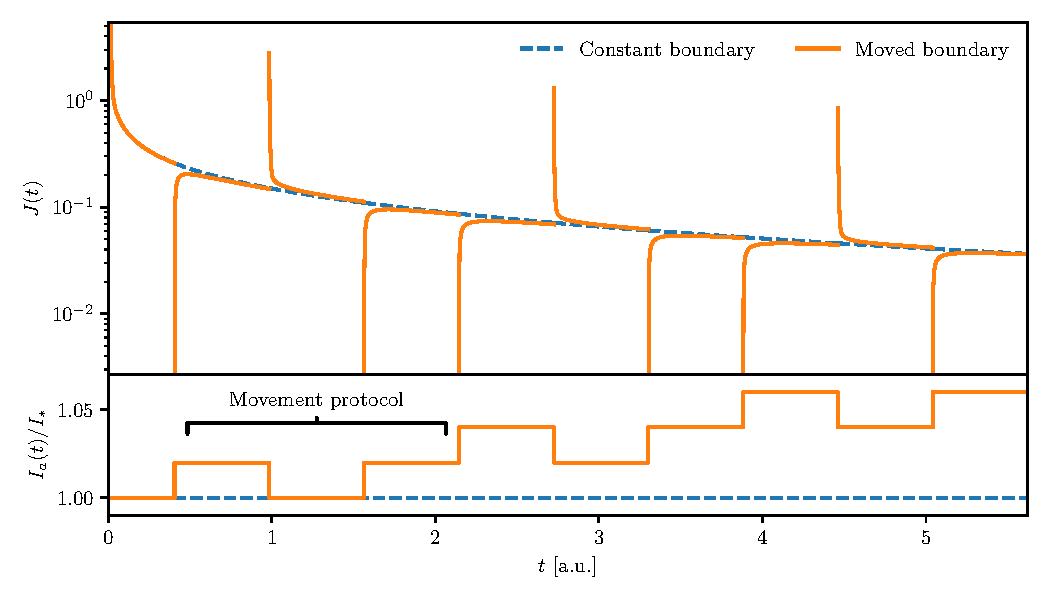
\includegraphics[width=\textwidth]{4_probing_the_diffusive_behavior/figs/final/the_protocol.pdf}
    \caption{Example of the proposed three-step protocol with a direct comparison between the condition with and without the variations in the position of the absorbing boundary condition. In this figure, the protocol is executed three times. The top plot shows the evolution of the outgoing current, while the bottom one shows the corresponding evolution of the position of the absorbing boundary condition. Note how the repetition of the three-step protocol moves progressively the absorbing boundary outwards. (Simulations parameters: $I_\ast = 1.0\,[\sigma^2],\,\kappa = 0.33$).}
    \label{fig:9}
\end{figure*}
%
\begin{figure*}[htp]
    \centering    
    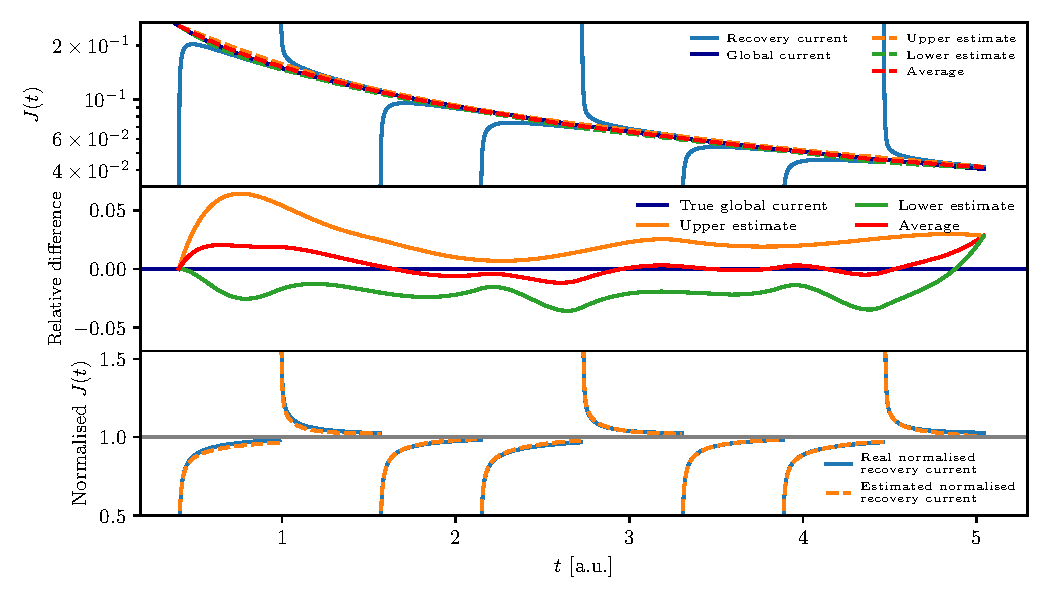
\includegraphics[width=\textwidth]{4_probing_the_diffusive_behavior/figs/final/the_interpolation.pdf}
    \caption{Example of the reconstruction process of the global current applied to a fraction of the data shown in Fig.~\ref{fig:9}. Top: Outgoing current from the process with constant boundary (dark blue) and with varying boundary conditions (light blue), along with the three components of the interpolation process. Middle: Relative difference, between the lower, average, or upper estimate of the global current and the true global current, of the interpolation procedure. Bottom: Comparison between the actual recovery current and the reconstructed one.}
    \label{fig:protocol}
\end{figure*}

%%%%%%%%%%%%%%%%%%%%%%%%%%%%%%%%%%%%%%%%%%%%%%%%%%%%%%%%%%%%%%%%%%%%%%%%%%%%%%%

\subsection{Reconstructing $D(I)$ from the normalized recovery currents}

%%%%%%%%%%%%%%%%%%%%%%%%%%%%%%%%%%%%%%%%%%%%%%%%%%%%%%%%%%%%%%%%%%%%%%%%%%%%%%%

After performing the proposed reconstruction protocol, a series of normalized recovery currents, obtained for different positions of the boundary condition, are available. All these curves are then used to reconstruct the shape of $D(I)$ via a fit procedure.

Thanks to the normalization procedure, every normalized recovery current can be considered as an individual and independent relaxation process, as in a system in equilibrium with a fixed source. Therefore, we can consider as expected current the convolution of the analytical current, presented in Eq.~\eqref{eq:thecurrent}, with one of our approximated difference distribution $\rho^\ast$, {according to Eq.~\eqref{eq:current_convolution}}. From a normalized recovery current obtained from an inward movement, we expect a relaxation curve characterized by an equivalent process with an initial distribution given by Eq.~\eqref{eq:inward_difference}, where the value of $\rho^\ast_\text{app}$ is computed considering $\alpha=1$, due to the normalization performed, the integral being computed over the appropriate action interval. Likewise, for a recovery current from an outward movement, we expect a curve characterized by an equivalent process with an initial distribution given by Eq.~\eqref{eq:outward_difference_approx}, where we consider $\gamma=1$, due to the normalization performed, the integral being computed over the appropriate action interval. Assuming a Nekhoroshev-like form for $D(I)$, the goal is to determine the values of the two parameters $I_\ast$ and $\kappa$, which is obtained by a standard non-linear least squares algorithm applied to the currents obtained during the execution of the proposed protocol. {The strong non-linearity of the functions involved in the least-square fit make the reconstruction of $I_\ast$ and $\kappa$ a difficult task, and alternative approaches have been tried. A possibility consists in performing a coarse scan of the $(I_\ast, \kappa)$ parameter space to identify an initial guess of the model parameters, and then perform a finer scan around the initial guess. In this approach, the distance between the numerical value of the recovery current and the one obtained from the analytical model for a given pair of $(I_\ast, \kappa)$ values is evaluated and the minimum provides either the initial guess of the parameters or their optimal value. This strategy has been successfully applied to the analysis of beam data reported in Ref.~\cite{montanari:ipac22-mopost043}. Another aspect of the fit is the strong correlation between the model parameters, typically of the order of a Pearson's product-moment coefficient of $0.9$, which is likely linked with the strongly non-linear function to be minimized. The impact of the strong correlation between the model parameters can be indeed mitigated by the approach based on parameters scanning rather than searching for the minimum with standard routines to perform numerical optimization.}

%%%%%%%%%%%%%%%%%%%%%%%%%%%%%%%%%%%%%%%%%%%%%%%%%%%%%%%%%%%%%%%%%%%%%%%%%%%%%%%%

\section{Numerical results}
\label{sec:numerical_results}

%%%%%%%%%%%%%%%%%%%%%%%%%%%%%%%%%%%%%%%%%%%%%%%%%%%%%%%%%%%%%%%%%%%%%%%%%%%%%%%%

To test the validity of the proposed procedure and to obtain a complete overview of its performance and limitations in the reconstruction of $D(I)$, several numerical simulations of diffusive processes with a Nekhoroshev-like diffusion coefficient have been performed by using the protocol described in Section~\ref{sec:moving_the_absorbing_barrier}. Particular emphasis is given to establishing the reliability of the proposed procedure as a function of the values of $\Delta I$ and $\Delta t$ used in the protocol of variation of the position of the boundary conditions.

%%%%%%%%%%%%%%%%%%%%%%%%%%%%%%%%%%%%%%%%%%%%%%%%%%%%%%%%%%%%%%%%%%%%%%%%%%%%%%%%

\subsection{Simulation parameters}

%%%%%%%%%%%%%%%%%%%%%%%%%%%%%%%%%%%%%%%%%%%%%%%%%%%%%%%%%%%%%%%%%%%%%%%%%%%%%%%%

As an initial condition, we consider the distribution in Eq~\eqref{eq:initial_distribution}, and we remark that all action variables are {dimensionless, and expressed either in units of beam sigma or in units of $I_\ast$}. We then consider a Nekhoroshev-like diffusive system characterized by the parameters obtained from the studies reported in Ref.~\cite{bazzani2020diffusion}, namely $I_\ast = 20.0\,[\sigma^2]$, $\kappa = 0.33$. Such a system, as it can be seen from Figs.~\ref{fig:1} and~\ref{fig:3}, is compatible with the semi-stationary regime and hence to the application of the proposed procedure.

Different values of the starting position $I_\mathrm{a}/I_\ast$ of the absorbing boundary condition have been considered. Even though most of our assumptions are valid for the $I_\mathrm{a}/I_\ast < 1$ regime, we consider also starting positions near $I_\ast$ and beyond $I_\ast$, i.e.\ in the saturation region of $D(I)$, to evaluate how robust the method is in non-ideal conditions.

For each configuration, after an initial time delay when a semi-stationary regime is reached, ten repetitions of the three-step protocol (outward-inward-outward), displayed in Fig.~\ref{fig:9}, have been performed. Several values of $\Delta I$, i.e.\ the action change of the boundary condition position, have been used to assess the presence of an optimal value for the reconstruction procedure. We remark that at the end of a simulation, the position of the absorbing boundary condition has moved from $I_\mathrm{a}/I_\ast$ to $(I_\mathrm{a} + 10\Delta I) / I_\ast$. 

Several values of the relaxation time $\Delta t$ have been considered to assess the reconstruction performance under different levels of equilibrium. We remark that an empirical relaxation time has been defined as the time for which a normalized recovery current is expected to recover the $99.9\%$ of the value of the original global current. Such an ideal time is computed using the full knowledge of $D(I)$, using our analytic current estimate Eq.~\eqref{eq:thecurrent}, and considering an outward movement of the absorbing boundary condition of size $\Delta I$ from the initial position of the absorbing boundary. It is stressed that, in general, we should assume that such relaxation time is not known when reconstructing the value of the diffusion coefficient. It is also worth mentioning that a criterion based on a complete $100\%$ recover of the global current cannot be used in practice, as this would require exponentially-long simulation times, needed to reach the relaxation of the inner part of the distribution, with negligible differences with respect to the $99.9\%$ case. Different fractions of this ideal time have been used when performing our procedure, and we evaluate how times shorter than the ideal relaxation time impact the quality of our final fit, as the system is still in a non-equilibrium regime when the next absorbing boundary movement occurs.

When working with the datasets generated by the various numerical simulations, a post-processing step on the normalized recovery currents is performed before executing the final fit procedure for reconstructing $D(I)$. It consists in selecting a fraction of the data representing the normalized recovery currents, i.e.\ only the normalized recovery current data up to a given percentage of the full recovery. For example, if we decide to filter out the normalized data beyond the $90\%$ recovery, it means that we discard values that are lower than $1.1$ for inward normalized recovery currents and values that are higher than $0.9$ for outward normalized recovering currents. We recall that, in the context of a normalized recovery current, a full recovery implies a value of $1.0$ as normalized recovery current.

This post-processing step is displayed in Fig.~\ref{fig:postprocessing}, where two different values of the fraction of the relaxation time between boundary movements are used in the numerical simulations. In both simulations, the boundary movement starts after an equal waiting time. In the left plot, the normalized recovery currents, reported already in Fig.~\ref{fig:protocol}, are shown together  with two different filtering levels. In the right plot, the same system is simulated using a shorter fraction of the relaxation time, and the recovery currents are shown together with the same filtering levels presented in the left plot. The much shorter time leads to only a partial recovery of the currents between boundary condition changes. For these sets of normalized recovery currents, the filtering levels displayed lead to almost no data reduction.
%
\begin{figure*}[htp]
    \centering 
    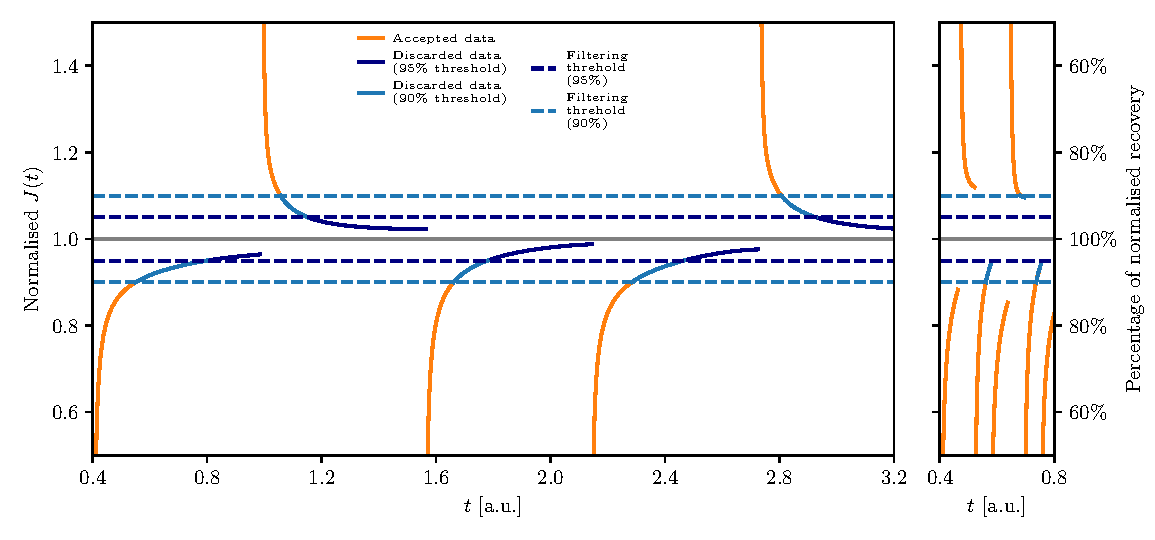
\includegraphics[width=\textwidth]{4_probing_the_diffusive_behavior/figs/final/the_discarded_data.pdf}
    \caption{Left: normalized recovery current, shown already in Fig.~\ref{fig:protocol}, together with two filtering levels. The boundary movements are performed after an initial evolution time $t=0.4 \, [\text{a. u.}]$, and the relaxation time $\Delta t$ between one boundary movement and the next one is equal to $\Delta t=0.58 \, [\text{a. u.}]$. Right: the same system is simulated with the same initial evolution time $t=0.4 \, [\text{a. u.}]$ and one order of magnitude shorter relaxation time $\Delta t=0.058 \, [\text{a. u.}]$, the resulting normalized recovery currents have not relaxed long enough to reach the $95\%$ filtering level. When the selected filtering level is not reached by the normalized recovery currents, the whole dataset is used for the fit reconstruction and no parts are discarded.}
    \label{fig:postprocessing}
\end{figure*}
%

By selecting different levels of filtering data, it is possible to evaluate how this choice affects the accuracy of the $D(I)$ reconstruction. It should be noted that our analytical approximation of Eq.~\eqref{eq:thecurrent} performs best when describing the evolution of a distribution near the absorbing boundary condition~\cite{montanari:ipac2021:tupab233}. Furthermore, the recovery current features an exponential-like decay that makes the analytical approximation less accurate over long timescales. For this reason, probing the dependence of the reconstruction performance on the fraction of data selected is very relevant.

%%%%%%%%%%%%%%%%%%%%%%%%%%%%%%%%%%%%%%%%%%%%%%%%%%%%%%%%%%%%%%%%%%%%%%%%%%%%%%%%

\subsection{Analysis of the reconstruction performance}

%%%%%%%%%%%%%%%%%%%%%%%%%%%%%%%%%%%%%%%%%%%%%%%%%%%%%%%%%%%%%%%%%%%%%%%%%%%%%%%%

The numerical exploration of the FP process entails a scan over several simulation parameters, leading to a large hyperspace of possible configurations. For this reason, we focus on the most ideal configurations, i.e.\ those that provide the best reconstruction performance, and then show how the other parameters affect the reconstruction accuracy of $I_\ast$ and $\kappa$.

After each execution of the proposed three-step protocol described in Section~\ref{sec:moving_the_absorbing_barrier} and shown in Fig.~\ref{fig:9}, we end up with two outward and one inward recovery currents. In every configuration explored, we observe better reconstruction results when considering only the recovery currents from the outward step. On the other hand, considering only the inward recovery currents or all currents simultaneously, poorer performance and numerical instabilities are observed. This is explained by the fact that when the position of the absorbing boundary is moved inwards, we are cutting in a distribution that is not necessarily in the perfect equilibrium configuration defined in our approximations. On the other hand, when we move the boundary condition outwards, we obtain a much more reliable observable of the distribution that populates the new available action interval, when evolving towards the new equilibrium state. It is possible to observe this behaviour in Fig.~\ref{fig:all_different_time}, where the relative error in the reconstruction of $\kappa$ and $I_\ast$ is shown for the three types of fit as a function of the fraction of the ideal relaxation time $\Delta t$ for two values of $I_\mathrm{a}/I_\ast$, representing the inner part of the stable-core region (left) and close to the change of regime of $D(I)$ (right). In the inner region, even small fractions of the relaxation time provide a good reconstruction of the fit parameters {(i.e.\ with a difference not greater than $10-15\%$)}. Furthermore, the three types of analysis, based on outward only, inward only, and inward and outward recovery currents provide results with comparable accuracy for longer fractions of the relaxation time.  
%
\begin{figure*}[htp]
    \centering
    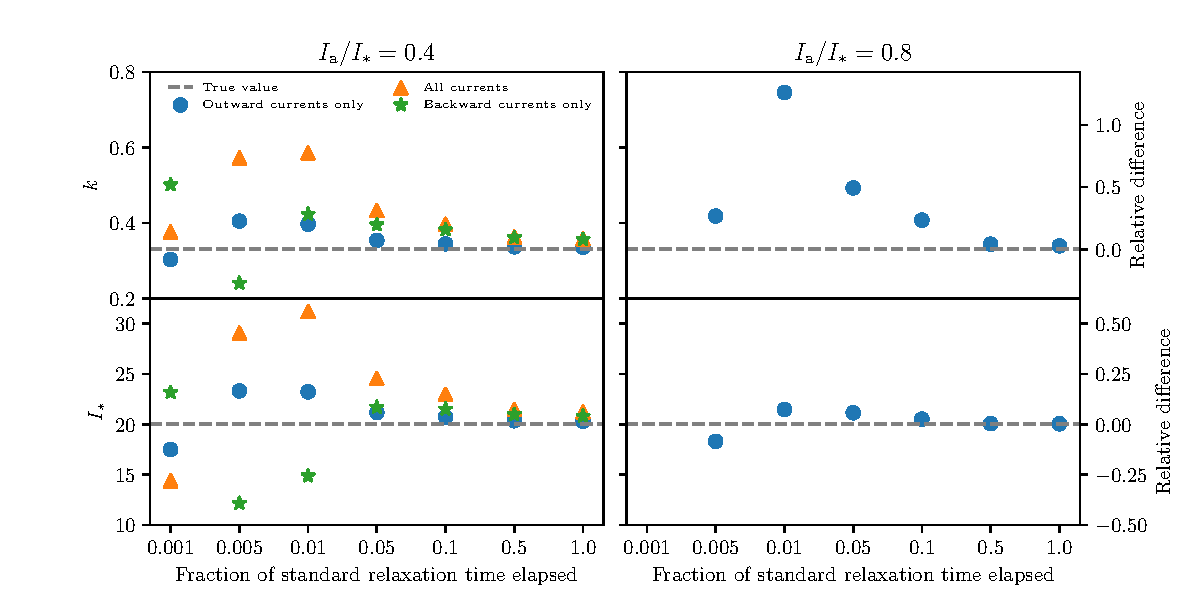
\includegraphics[width=\textwidth]{4_probing_the_diffusive_behavior/figs/final/better_plot.pdf}
    \caption{Fit results for $I_\ast$ and $\kappa$ as a function of the relaxation time $\Delta t$ for two values of $I_\mathrm{a}/I_\ast$, using different subsets of the numerical data. Left: for $I_\mathrm{a}/I_\ast=0.4$, a good reconstruction performance  {(i.e.\ with a difference not greater than $20\%$)} is observed even for short fractions of the ideal relaxation time. A rather similar performance is observed for the three types of analysis, the one based on the outward currents having the best performance. Right: for $I_\mathrm{a} / I_\ast=0.8$, only the cases corresponding to longer fractions of the relaxation time feature a good performance. Moreover, only the analysis based on the outward currents is displayed, as the other two features either failures or large errors in the fit. (Simulation parameters: initial $I_\mathrm{a}/I_\ast=0.4$, boundary step $\Delta I =0.1 \sigma^2$, 10 repetitions of the three-step procedure, data up to a maximum current recovery of $90\%$).}
    \label{fig:all_different_time}
\end{figure*}
%

In the transition region, however, only longer fractions of the relaxation time provide a good reconstruction of the fit parameters  {(i.e.\ with a difference not greater than $20\%$)} and the only applicable type of analysis is the one based on the outward recovery currents. The other two analyses feature either failures or larger errors in the fit, {which are generated by the behaviour of the inward recovery current}. Based on the observed behaviour, in the next plots we will only display results from the reconstruction based on the outward recovery currents. {The reasons for the poor performance of the reconstruction of $I_\ast$ and $\kappa$ whenever inward recovery currents are considered is at least twofold. The first reason stems from the fact that by cutting the distribution with the inward movement of the boundary condition the system enters a non-equilibrium regime, in which the recovery current features sizeable variations. If enough time is elapsed, the system reaches a new equilibrium and the recovery current is much more reliable for the reconstruction of $I_\ast$ and $\kappa$, as observed in Fig.~\ref{fig:all_different_time}. The second reason is of purely numerical origin, but somewhat linked to the first one, as when an inward step is performed, the equilibrium distribution is cut and the sharp edge needs to be smoothed by applying a logistic function to the cut distribution (see the discussion in Appendix~\ref{app_sec:numerical_integration_with_crank_nicolson}). This has potential harmful effects on the generated recovery current, subsequently used to reconstruct the model parameters. Note that the first argument is even more applicable to the case of data from beam experiments, as observed from the data analyses carried out recently and discussed in Ref.~\cite{montanari:ipac22-mopost043}.}

In Fig~\ref{fig:different_position}, the reconstruction error for the two fit parameters as a function of the starting position of the absorbing boundary $I_\mathrm{a}/I_\ast$ is shown. 
%
\begin{figure*}[htp]
    \centering
    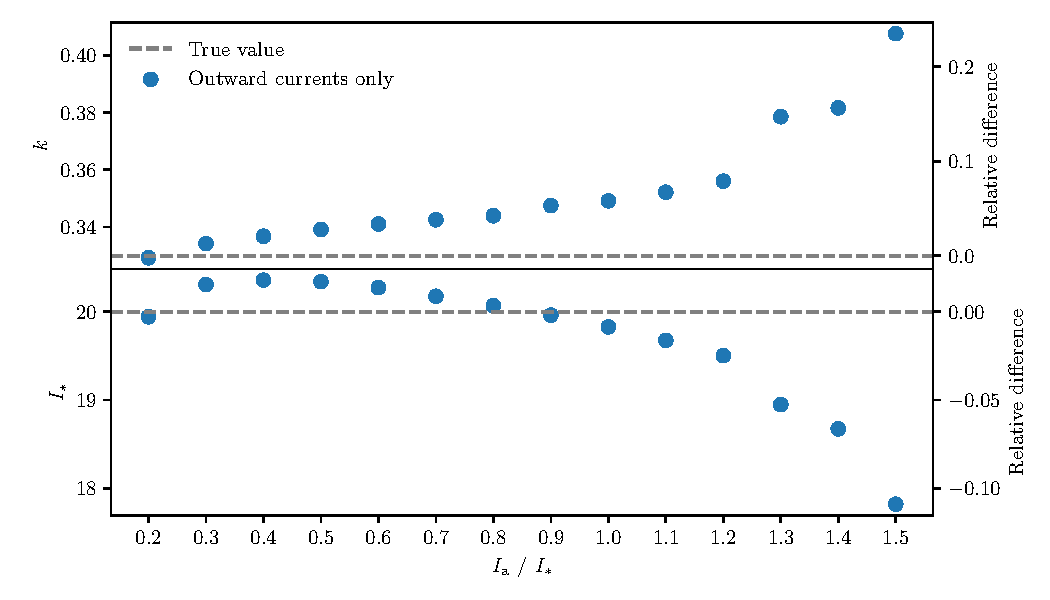
\includegraphics[width=\textwidth]{4_probing_the_diffusive_behavior/figs/final/different_position.pdf}
    \caption{Fit results for $I_\ast$ and $\kappa$ as a function of the initial value of $I_\mathrm{a}/I_\ast$. The reconstruction performance is excellent for $I_\mathrm{a}/I_\ast \leq 1$, while for larger values the relative error increases. (Simulation parameters: boundary step $\Delta I=0.1 \sigma^2$, relaxation time $\Delta t=0.5$, 10 repetitions of the three-step procedure, data up to a maximum current recovery of $90\%$).}
    \label{fig:different_position}
\end{figure*}
%
The performance is excellent for $I_\mathrm{a}/I_\ast \leq 1$ {(i.e.\ with a difference not greater than $5\%$)}, whereas outside this region the reconstruction error increases. This behaviour is to be expected, as a recovery current carries mainly local information about $D(I)$. Hence, if only the region $I_\mathrm{a}/I_\ast > 1$ is sampled, the information about $D(I)$ reflects only its quasi-linear regime (see Fig.~\ref{fig:1}). Such incomplete information inevitably affects the performance of the final fit, as it prevents an accurate reconstruction of the strongly non-linear part of the diffusion coefficient. This result suggests also that, after having determined the fit parameters, one can verify whether the action interval explored was suitable for an accurate reconstruction of the functional form of the diffusion coefficient.

The plots in Fig.~\ref{fig:different_position} provide some insight on the dependence of the reconstruction performance as a function of a single parameter while the others are kept fixed. In the following figures, however, the relative error of the reconstruction procedure is shown as a function of two parameters. The colour code represents the relative difference between the reconstructed (from the proposed protocol) and the true (used in the numerical simulations of the FP processes) values of $I_\ast$ and $\kappa$ that describe $D(I)$. The scale is limited to a $20\%$ relative difference, which is assumed as a threshold to identify a poor performance. Note that white cells represent cases in which the reconstruction procedure failed.

Figure~\ref{fig:different_cut} shows the relative error as a function of the cut of the recovery current performed during the post-processing and $I_\mathrm{a}/I_\ast$. The performance of the reconstruction approach improves when the recovery currents are cut. This depends on the fact that our approach is local, i.e.\ accurate to describe the system's behaviour close to the boundary condition. The longer the recovery time, the less local is the information gathered from the current. For this reason, the plots concerning the reconstruction performance are based on recovery currents cut at $90\%$. 

\begin{figure*}[htp]
    \centering
    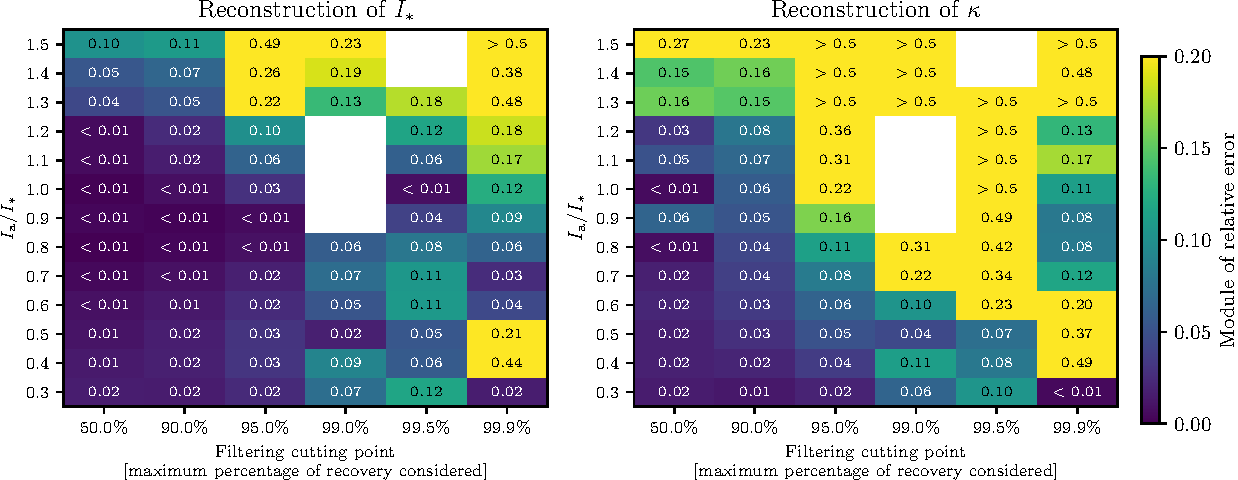
\includegraphics[width=\textwidth]{4_probing_the_diffusive_behavior/figs/final/MULTI_different_filter.pdf}
    \caption{2D view of the reconstruction performance as a function of the cut in the recovery current, as applied in Fig.~\ref{fig:postprocessing}, and of the initial value of $I_\mathrm{a}/I_\ast$. It is clearly seen how certain values of the cut provide a consistent increase in reconstruction performance. White regions indicate a failure in convergence in the final fit procedure. (Simulation parameters: relaxation time $\Delta t=1$, boundary step $\Delta I=0.1 \sigma^2$, 10 repetitions of the three-step, data up to a maximum current recovery of $90\%$).}
    \label{fig:different_cut}
\end{figure*}

As for the reconstruction performance as a function of the  relaxation time $\Delta t$, Fig.~\ref{fig:different_time} shows the behaviour including the dependence on $I_\mathrm{a}/I_\ast$. In this case, the longer the relaxation time, the better is the performance of the reconstruction. In particular, longer relaxation times allow a better reconstruction even for large values of $I_\mathrm{a}/I_\ast$. It is worth highlighting that in the case of short relaxation times, a good overall performance can be achieved only by working at $I/I_\ast \ll 1$.
%
\begin{figure*}[htp]
    \centering
    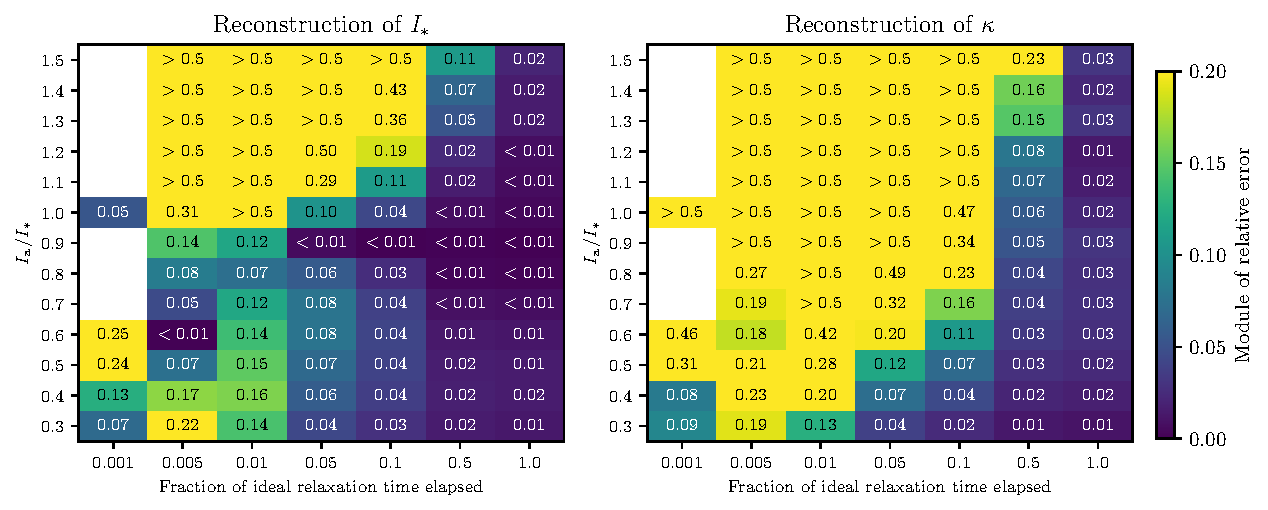
\includegraphics[width=\textwidth]{4_probing_the_diffusive_behavior/figs/final/MULTI_different_time.pdf}
    \caption{2D view of the reconstruction performance as a function of the relaxation time $\Delta t$ and the initial value of $I_\mathrm{a}/I_\ast$. It is clearly seen how the reconstruction performance improves for longer relaxation times. However, the method proves to be rather robust for fractions of ideal time up to $5\%$ provided $I_\mathrm{a}/I_\ast < 0.6$. White regions indicate a failure in convergence in the final fit procedure. (Simulation parameters: boundary step $\Delta I=0.1 \sigma^2$, 10 repetitions of the three-step procedure, data up to a maximum current recovery of $90\%$, if smaller values of $\Delta t$ lead to a normalized recovery below $90\%$, all the normalized recovery current data are used for the reconstruction).}
    \label{fig:different_time}
\end{figure*}
%
Combining the results of the last two analyses, one concludes that the best approach for an accurate determination of $I_\ast$ and $\kappa$ consists in increasing the relaxation time between successive changes of the position of the boundary condition and cutting the data from the recovery currents. 

Figure~\ref{fig:different_nsamples} shows the 2D plot of the reconstruction performance as a function of the number of repetitions of the three-step procedure and $I_\mathrm{a}/I_\ast$. It can be seen with the higher number of repetitions, how the performance improves. This is naturally linked to the fact that repeating the three-step procedure implies sampling a larger extent of phase space, thus probing more accurately the behaviour of the diffusion coefficient as a function of the action. It is also clearly visible that starting from six repetitions of the three-step procedure, a good reconstruction is obtained for $I_\mathrm{a}/I_\ast < 1$.

\begin{figure*}[htp]
    \centering
    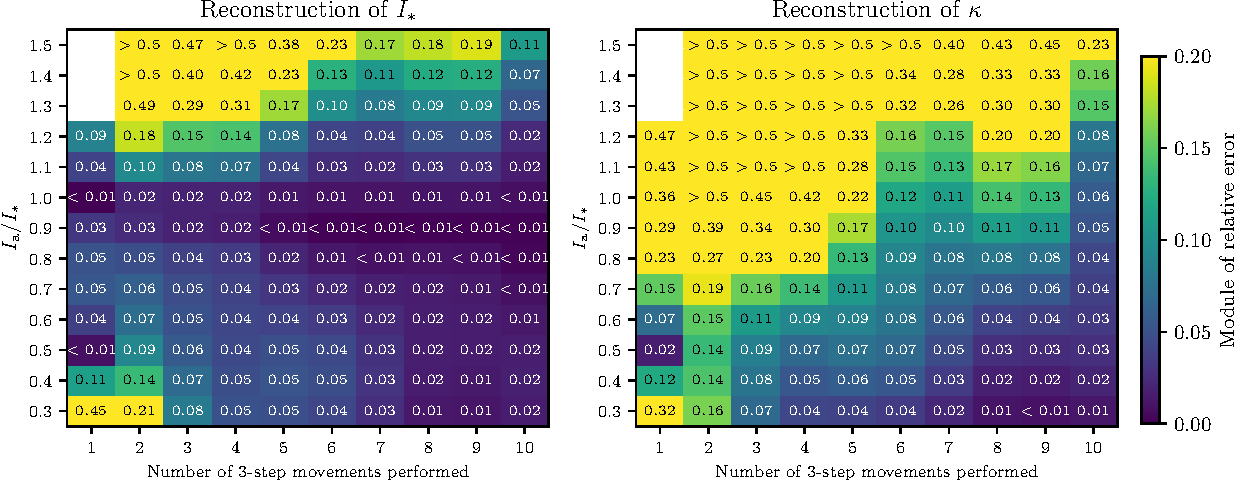
\includegraphics[width=\textwidth]{4_probing_the_diffusive_behavior/figs/final/MULTI_different_samples.pdf}
    \caption{2D view of the reconstruction performance as a function of the number of three-step movements and of $I_\mathrm{a}/I_\ast$ starting positions. It is clearly seen how the performance increases with the number of three-step movements, as larger regions of phase space are explored (as in Fig.~\ref{fig:9}). White regions indicate a failure in convergence in the final fit procedure. (Simulation parameters: relaxation time $\Delta t=0.5 \, [\text{a. u.}]$, boundary step $\Delta I=0.1 \sigma^2$, which is $\Delta I / I_\ast = 0.005$, data up to a maximum current recovery of $90\%$ is considered).}
    \label{fig:different_nsamples}
\end{figure*}

Finally, the impact of $\Delta I$ is shown in Fig.~\ref{fig:different_movement_module}, where the performance as a function of $\Delta I$ and $I_\mathrm{a}/I_\ast$ is depicted.  We see how the performance is not strongly affected by the choice of $\Delta I$, i.e.\ relative error fluctuations are less than $10\%$ for differences of an order of magnitude in $\Delta I$. However, it is important to highlight two facts that might suggest a choice in the size of the change of position of the absorbing boundary condition: (1) the ideal relaxation time is directly proportional to the size of the absorbing boundary movement; (2) a too small $\Delta I$ might lead to a too local sampling in action space, thus negatively affecting the final reconstruction of $D(I)$. 

\begin{figure*}[htp]
    \centering
    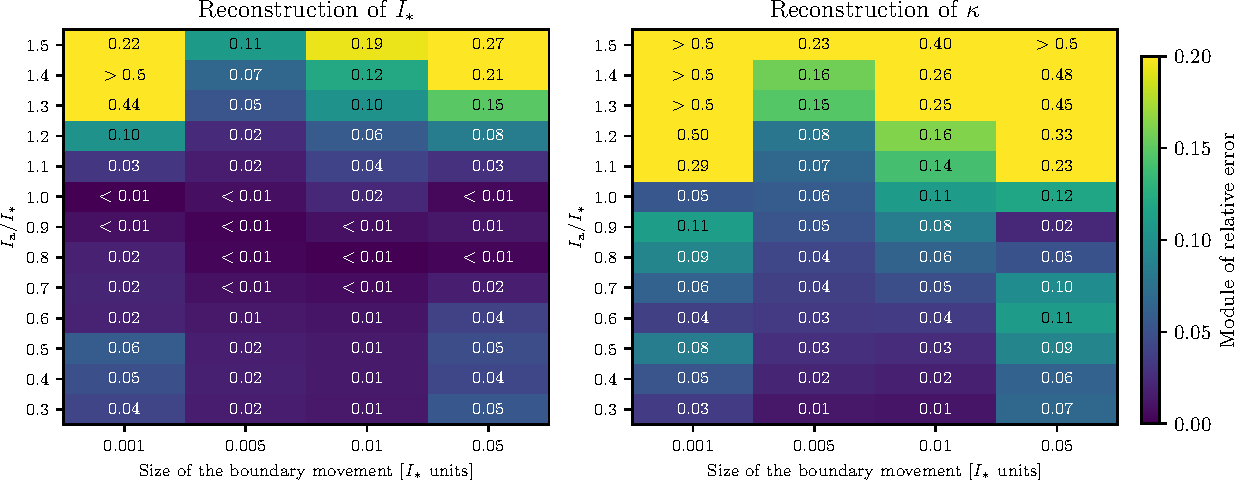
\includegraphics[width=\textwidth]{4_probing_the_diffusive_behavior/figs/final/MULTI_different_step_size.pdf}
    \caption{2D view of the reconstruction performance as a function of $\Delta I$ and $I_\mathrm{a}/I_\ast$. The  best performance is achieved for $\Delta I = 0.005 \sigma^2$, but the dependence on $\Delta I$ is very weak (Simulation parameters: relaxation time $\Delta t=0.5 \, [\text{a. u.}]$, 10 repetitions of the three-step procedure, data up to a maximum current recovery of $90\%$).}
    \label{fig:different_movement_module}
\end{figure*}

%%%%%%%%%%%%%%%%%%%%%%%%%%%%%%%%%%%%%%%%%%%%%%%%%%%%%%%%%%%%%%%%%%%%%%%%%%%%%%%%

\section{Final remarks}
\label{sec:conclusions}

%%%%%%%%%%%%%%%%%%%%%%%%%%%%%%%%%%%%%%%%%%%%%%%%%%%%%%%%%%%%%%%%%%%%%%%%%%%%%%%%

Beam-halo scans, performed with movable collimators jaws, have been used intensively for probing the diffusive behaviour of the beam halo in circular accelerators and seems a very useful tool for probing this special regime of beam dynamics in the absence of beam instrumentation capable of providing diagnostic tools to study beam-halo dynamics.

{The main result of this Chapter} is the identification of an efficient protocol for probing the shape of {a diffusion coefficient consistent with the stability time estimate of Nekhoroshev theorem}. The protocol has been scrutinized by means of detailed numerical simulations, {but} it is clear that eventually it should be tested with beam measurement data. Two aspects should be highlighted: although the framework presented in this article is one-dimensional, i.e.\ considering non-linear beam dynamics in one degree of freedom, we believe that it can be applied to cases representing systems with two degrees of freedom (as shown in Ref.~\cite{bazzani2020diffusion}). Furthermore, the proposed approach does not rely on a previous knowledge of the beam distribution, which is a clear advantage for applications. 
 
The proposed protocol relies on the idea that it is possible to separate the measured outgoing current into a global current, i.e.\ the general outgoing current loss that is measured from the exponentially slow erosion of the stable core of the beam, and a recovery current, i.e.\ the current following a change of the position of the boundary condition, which corresponds to a non-equilibrium state. By performing an alternating three-step sequence of outward-inward-outward boundary-condition changes, which can easily be done by means of collimator scans, it is possible to reconstruct the global current of the erosion process and use that to normalize the recovery currents. Each normalized recovery current ultimately contains local information on the diffusion coefficient without the need of prior knowledge on the form of the initial distribution in action space, and can be used for estimating its global shape.

The performance of this protocol has been tested by means of many numerical simulations of Fokker-Planck processes performed in various configurations, to evaluate the reliability and limits of our approach. The protocol proved to be capable of reconstructing with precision and good accuracy  {(i.e.\ with an error not greater than $10-15\%$)} the parameters of the diffusion coefficient when it is performed in a phase-space region where the diffusion coefficient has an exponential evolution, i.e.\ for $I/I_\ast < 1$, the relaxation time between boundary condition changes is long enough so that the system reaches an equilibrium state, and multiple amplitudes have been probed. For this last condition, the optimal number of amplitudes to be sampled is highly dependent on the detail of the diffusion process, however, from the simulations it appears that about six sequences of three-step absorbing boundary changes covering the $I / I_\ast < 1$ region is a good choice. 

The analysis also highlighted how a good reconstruction performance can be achieved by considering only the outgoing recovery currents in the final fitting reconstruction, and by discarding part of the recovery current data beyond a certain level, as it is more prone to reconstruction errors and more difficult to characterize with our analytical formulas. It is worth stressing that the reconstruction performance proves to be good even if the optimal conditions are not fully met. Most importantly, the procedure provides useful information about possible shortcomings present in the dataset under consideration, such as a high uncertainty band in the global current reconstruction, or a reconstructed value of $I_\ast$ that indicates that the probed phase-space region is outside the optimal interval $I / I_\ast < 1$. In these cases, the protocol should be reapplied in better conditions, e.g.\ by adjusting the range of actions probed to satisfy the condition $I / I_\ast < 1$.

Thanks to the positive and encouraging results of the analysis presented here, we are confident that the measurement protocol is a powerful tool for probing the non-linear diffusive behaviour in an accelerator like the LHC, although it should be stressed that it is of general applicability in any circular accelerator. Therefore, the logical next step is the proposal of a dedicated beam measurement, at the LHC or elsewhere, performed in the optimal conditions considered in this Chapter, which will complete the investigations presented in this Chapter. In the meantime, available data from collimator scans collected at the LHC (but not with the proposed protocol), have been analysed under the assumption of the proposed functional form for the diffusion coefficient. Very promising results have been obtained that support pursuing this line of research, and will be presented in the next Chapter.